\section{HTML Imports}\label{html-imports}

Bisher erlauben es praktisch alle Plattformen, Codeteile zu Importieren und zu verwenden, nur nicht das Web, bzw. \ac{HTML}. Das heutige \ac{HTML} ermöglicht es externe Stylesheets, JavaScript Dateien, Bilder etc. in ein \ac{HTML} Dokument zu importieren, \ac{HTML}-Dateien selbst können jedoch nicht importiert werden. Auch ist es nicht möglich, alle benötigten Dateien in einer Ressource zu bündeln und als einzige Abhängigkeit zu importieren. \ac{HTML} Imports versuchen eben dieses Problem zu lösen. So soll es möglich sein, \ac{HTML}-Dateien und wiederum \ac{HTML}-Dateien in \ac{HTML}-Dateien zu importieren. So können auch verschiedene benötigte Dateien in einer \ac{HTML}-Datei gesammelt und mit nur einem Import in die Seite eingebunden werden. Doppelte Abhängigkeiten sollen dadurch automatisch aufgelöst werden, sodass Dateien, die mehrmals eingebunden werden sollten, automatisch effektiv nur einmal heruntergeladen werden.


\subsection{HTML-Dateien importieren}\label{html-dateien-importieren}

Imports von \ac{HTML}-Dateien werden, wie andere Imports auch, per \texttt{\textless{}link\textgreater{}}-Tag deklariert. Neu ist jedoch der Wert des \texttt{rel}-Attributes, welches auf \texttt{import} gesetzt wird \cite[S. 139-147]{citeulike:13844975}. So kann beispielsweise das Bootstrap-Framework statt wie bisher mit mehreren Imports mit nur einem Import eingebunden werden. Bisher könnte die Einbindung unter Berücksichtigung der Abhängigkeiten wie in Listing \ref{evbohtmli} aussehen.

\lstinputlisting[language=HTML,label=evbohtmli,caption=Einbindung von Bootstrap ohne \ac{HTML} Imports]{kapitel2/listings/5-1.html}

Stattdessen kann dieses Markup nun in ein einziges \ac{HTML} Dokument, welches alle Abhängigkeiten verwaltet, geschrieben werden. Dieses wird dann mit einem einzigen Import \texttt{\textless{}link\ rel=\dq import\dq\ href=\dq bootstrap.html\dq\textgreater{}} in das eigene \ac{HTML} Dokument importiert.

Es ist jedoch zu beachten, dass \ac{HTML} Imports nur auf Ressourcen der gleichen Quelle, also dem gleichen Host, respektive der gleichen Domain zugreifen können. Imports von \ac{HTML}-Dateien von verschiedenen Quellen stellen eine Sicherheitslücke dar, da Webbrowser die \ac{SOP} verfolgen.

\begin{quote}
The same-origin policy restricts how a document or script loaded from one origin can interact with a resource from another origin. It is a critical security mechanism for isolating potentially malicious documents. \cite{citeulike:13853253}
\end{quote}

Sollte das jedoch dennoch erlaubt werden, so muss das \ac{CORS} für die entsprechende Domain auf dem Server aktiviert werden.

\begin{quote}
These restrictions prevent a client-side Web application running from one origin from obtaining data retrieved from another origin, and also limit unsafe \ac{HTTP} requests that can be automatically launched toward destinations that differ from the running application's origin. \cite{citeulike:13853643}
\end{quote}


\subsection{Auf importierte Inhalte zugreifen}\label{html-imports-verwenden}

Importierte \ac{HTML}-Dateien werden nicht nur in das Dokument eingefügt, sondern vom Parser verarbeitet, das bedeutet, dass mit JavaScript auf das \ac{DOM} des Imports zugegriffen werden kann. Wenn sie vom Parser verarbeitet worden sind, sind sie zwar verfügbar, allerdings werden die Inhalte nicht angezeigt bis sie mittels JavaScript in das \ac{DOM} eingefügt werden. Ihre enthaltenen Scripte werden also ausgeführt, Styles und \ac{HTML}-Knoten werden jedoch ignoriert. Um nun die Inhalte eines Imports auf der Seite einzubinden, muss auf die \texttt{.import} Eigenschaft des \texttt{\textless{}link\textgreater{}}-Tags mit dem Import zugegriffen werden \texttt{var\ content\ =\ document.querySelector('link{[}rel=\dq import\dq{]}').import;}. Nun kann auf das \ac{DOM} des Imports zugegriffen werden. So kann ein enthaltenes Element mit der Klasse \texttt{element} mit \texttt{var\ el\ =\ content.querySelector('.element');} geklont und anschließend durch \texttt{document.body.appendChild(el.cloneNode(true));} in das eigene \ac{DOM} eingefügt werden. Falls es jedoch mehrere Imports geben sollte, können den Imports IDs zugewiesen werden, anhand derer die Imports voneinander unterschieden werden können (siehe Listing \ref{euvvhtmli}) \cite{citeulike:13853724}.

\lstinputlisting[language=HTML,label=euvvhtmli,caption=Einbinden und Verwenden von \ac{HTML} Imports]{kapitel2/listings/5-2.html}


\subsection{Abhängigkeiten verwalten}\label{abhuxe4ngigkeiten-verwalten}

Jedoch kann es vor kommen, dass mehrere eingebundenen Bibliotheken die gleichen Abhängigkeiten haben und diese verwaltet werden müssen. Sollte dies nicht sorgfältig gemacht werden, können unerwartete Fehler auftreten, die mitunter nur schwer zu lokalisieren sind. \ac{HTML} Imports verwalten Abhängigkeiten automatisch. Um das zu erreichen, werden die Abhängigkeiten gebündelt und in eine zu importierende \ac{HTML}-Datei geschrieben. Haben mehrere Imports die gleichen Abhängigkeiten (siehe Listing \ref{ahvmhtmli}), werden diese vom Browser erkannt und nur einmal heruntergeladen. Mehrfachdownloads und Konflikte der Abhängigkeiten werden so verhindert \cite{citeulike:13853700}.

\lstinputlisting[language=HTML,label=ahvmhtmli,caption=Abhängigkeitsverwaltung mit \ac{HTML} Imports]{kapitel2/listings/5-3.html}

Selbst wenn die jQuery-Library in mehreren Dateien eingebunden wird, wird hier sie dennoch nur einmal übertragen. Wenn nun fremde \ac{HTML}-Dateien eingebunden werden muss auch nicht auf die auf die Reihenfolge der Imports geachtet werden, da diese selbst ihre Abhängigkeiten beinhalten.


\subsection{Sub-Imports}\label{sub-imports}

Das obige Beispiel zeigt, dass \ac{HTML} Imports selbst wiederum auch \ac{HTML} Imports beinhalten können. Diese Imports werden Sub-Imports genannt und ermöglichen einen einfachen Austausch oder eine Erweiterungen von Abhängigkeiten innerhalb einer Komponente. Wenn eine Komponente A eine Abhängigkeit von einer Komponenten B hat und eine neue Version von Komponente B verfügbar ist, kann dies einfach in dem Import des Sub-Imports angepasst werden ohne den Import in der Eltern-\ac{HTML}-Datei anpassen zu müssen \cite{citeulike:13853647}.


\subsection{Performance}\label{html-import-performance}

Ein signifikantes Problem der \ac{HTML} Imports ist die Performance, welche bei komplexen Anwendungen schnell abfallen kann. Werden auf einer Seite mehrere Imports eingebunden, die selbst wiederum Imports beinhalten können, so steigt die Anzahl an Requests an den Server schnell exponentiell an, was die Webseite stark verlangsamen kann. Auch das vorkommen von doppelten Abhängigkeiten kann die Anzahl an Requests in die Höhe treiben, doch da Browser die Abhängigkeiten nativ schon selbst de-duplizieren, kann dieses Problem in diesem Zusammenhang ignoriert werden \cite{citeulike:13853714}.

Dennoch sind viele Einzel-Requests ein gewünschtes Verhalten von Web Components, da sie bereits mit Blick auf Version 2 des \ac{HTTP}-Protokolls entwickelt wurden. In diesem können mehrere Requests in einer \ac{TCP}-Verbindung übertragen werden. Des Weiteren kann der Client die Priorität der angeforderten Dateien bestimmen, um Dateien mit einer hohen Priorität vor Dateien mit niedrigerer Priorität zu erhalten. Ebenso wird mit einer neuen Header-Kompression die zu übertragende Datenmenge verkleinert. Neu sind außerdem die sogenannten ``Server Pushes'', welche es dem Server ermöglichen, Nachrichten an den Client zu schicken, ohne dass dieser sie anfordern muss.

Voraussetzung hierfür ist jedoch die Unterstützung des neuen Protokolls seitens des Browsers. Bis auf den Internet Explorer und Safari unterstützen jedoch alle Browser \ac{HTTP}/2 schon ab frühen Versionen, allerdings nur bei mittels \ac{TLS} verschlüsselten Webseiten [citeulike:13879562]. Der Anteil der über \ac{HTTP}/2 ausgelieferten Webseiten liegt momentan bei circa 3\% \cite{citeulike:13879575}.


\subsection{Asynchrones Laden von Imports}\label{asynchrones-laden-von-imports}

Das Rendern der Seite kann unter Umständen sehr lange dauern, da das in den Imports enthaltene JavaScript das Rendern blockiert. Um das zu verhindern und alle Dateien möglichst schnell laden zu können, ist ein \texttt{async}-Attribut vorgesehen. Dieses funktioniert jedoch nur, wenn als Protokoll \ac{HTTP}/2 gewählt wird. Das Attribut ermöglicht es, dass mehrere Dateien asynchron geladen werden können. In den Imports enthaltenes JavaScript blockiert somit nicht das Rendern von bereits geladenem \ac{HTML} Code. Falls \ac{HTTP}/2 nicht vorhanden sein sollte, kann alternativ das \texttt{defer}-Attribut gewählt werden, wodurch das JavaScipt erst nach vollständigem Parsen des \ac{HTML} ausgeführt wird. Eine weitere Methode ist das Laden der Imports am Ende der Seite. Somit wird sichergestellt, dass die Scripte erst ausgeführt werden, wenn die Seite geladen und gerendert wurde.


\subsection{Anwendungen}\label{anwendungen}

Besonders einfach machen \ac{HTML} Imports das Einbinden ganzer Web Applikationen mit \ac{HTML}/JavaScript/\ac{CSS}. Diese können in eine Datei geschrieben, ihre Abhängigkeiten definieren und von anderen importiert werden. Dies macht es sehr einfach, den Code zu organisieren, so können etwa einzelne Abschnitte einer Anwendung oder von Code in einzelne Dateien ausgelagert werden, was Web Applikationen modular, austauschbar und wiederverwendbar macht. Falls nun ein oder mehrere Custom Elements in einem \ac{HTML} Import enthalten sind, so werden dessen Interface und Definitionen automatisch gekapselt. Auch wird die Abhängigkeitsverwaltung in Betracht auf die Performance stark verbessert, da der Browser nicht eine große JavaScript-Library, sondern einzelne kleinere JavaScript-Abschnitte parsen und ausführen muss. Diese werden durch die \ac{HTML} Imports parallel geparst, was mit einen enormen Performance-Schub einher geht \cite{citeulike:13853647}.


\subsection{Browserunterstützung}\label{browserunterstuxfctzung}

\ac{HTML} Imports sind noch nicht vom \ac{W3C} standardisiert, sondern befinden sich noch im Status eines ``Working Draft'' \cite{citeulike:13853711}. Sie werden deshalb bisher nur von Google Chrome ab Version 43 und Opera ab Version 33 nativ unterstützt (siehe Abbildung \ref{fig:bdhtmli}). Seitens Mozilla und dessen Browser Firefox wird es für \ac{HTML} Imports auch keine Unterstützung geben, da ihrer Meinung nach der Bedarf an \ac{HTML} Imports nach der Einführung von ECMAScript 6 Modules nicht mehr existiert und da Abhängigkeiten schon mit Tools wie Vulcanize aufgelöst werden können \cite{citeulike:13881144}. Auf Details zu ECMAScript 6 Modules wird an dieser Stelle nicht eingegangen, da diese den Umfang dieser Arbeit überschreiten.

\begin{figure}[htbp]
 \centering
 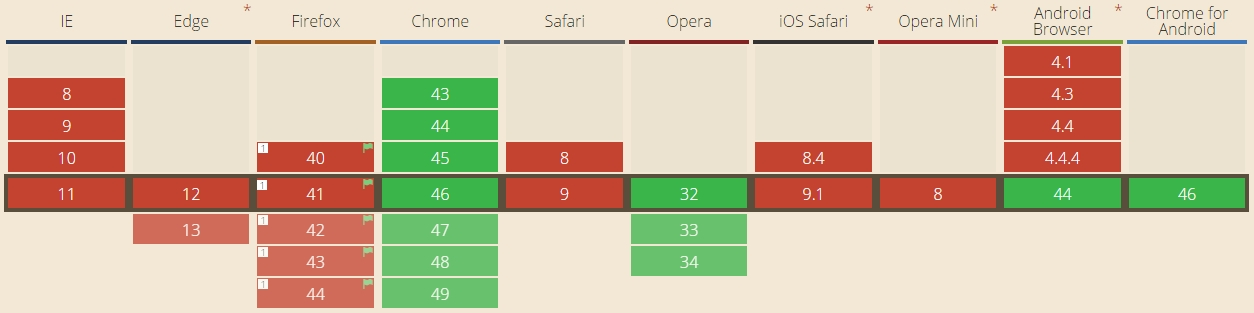
\includegraphics[width=\linewidth]{kapitel2/bilder/5-html-imports-browserunterstuetzung}
 \caption{Browserunterstützung der HTML Imports}
 \label{fig:bdhtmli}
\end{figure}

